\documentclass[a4paper,11pt]{article}
\usepackage{a4wide}
\usepackage{fullpage}
\usepackage[utf8x]{inputenc}
\usepackage[slovene]{babel}
\selectlanguage{slovene}
\usepackage[toc,page]{appendix}
\usepackage[pdftex]{graphicx} % za slike
\usepackage{setspace}
\usepackage{color}
\definecolor{light-gray}{gray}{0.95}
\definecolor{green}{RGB}{0,128,0}
\usepackage{listings} % za vključevanje kode
\usepackage{hyperref}
\renewcommand{\baselinestretch}{1.2} % za boljšo berljivost večji razmak
\renewcommand{\appendixpagename}{Priloge}

\lstset{ % nastavitve za izpis kode, sem lahko tudi kaj dodaš/spremeniš
language=c++,
basicstyle=\footnotesize,
basicstyle=\ttfamily\footnotesize\setstretch{1},
backgroundcolor=\color{light-gray},
}

\title{RIS - Poročilo}
\author{Jan Gulič, Luka Podgoršek, Rok Poje, Sašo Cvitkovič}
\date{\today}

\begin{document}

\maketitle
% ----------------------------- UVOD ---------------------------------------- %
\section{Uvod}

Pri predmetu Razvoj inteligentnih sistemov (RIS) smo ekipo z imenom \textbf{team theta} sestavljali:
\begin{itemize}
	\item Jan Gulič
	\item Luka Podgoršek
	\item Rok Poje
	\item Sašo Cvitkovič
\end{itemize}

% ----------------------------- OPIS PROBLEMA ---------------------------------------- %

\section{Opis problema}

Končna naloga je bila implementacija robotskega taksija. Poligon je predstavljal mesto, v katerem se je robot vozil in izpoljeval naloge. Mesto je bilo sestavljeno iz štirih ulic, štirih hiš in prometnih znakov, katere je robot moral upoštevati med samo vožnjo. Na začetku smo robota postavili v mesto in mu sporočili njegovo lokacijo. Nato je uporabnik preko telefona (uporabljena je bila Android aplikacija) sporočil robotu svoje ime in na kateri ulici se nahaja. Robot se je odpeljal na željeno ulico in poiskal uporabnika, ki ga je poklical. Nato je s potnikom opravil kratek dialog, preko katerega je izvedel željeno destinacijo. Uporabnika je odpeljal na destinacijo, kjer je moral poiskati stavbo. Stavbe so bile predstavljene kot barvni cilindri. Po uspešni dostavi se je robot odpeljal po naslednjega uporabnika. 
Robot je nalogo opravil, ko je uspešno odpeljal tri osebe na željeno destinacijo.\\


Slike mesta, obrazev in zgradb najdete v prilogi \ref{sec:slike}.

% ----------------------------- OPIS GLAVNIH NALOG ---------------------------------------- %

\subsection{Opis glavnih nalog -- REMOVE}
\subsubsection{Detekcija in razpoznava}
Robot je moral zaznati in razpoznati osebe, prometne znake in zgradbe.
\subsubsection{Dialog z osebo}
Robot je moral preko dialoga z osebo razpoznati ukaze in jih nato izvesti.
\subsubsection{Navigacija}
Robot se je moral znati navigirati v vnaprej pripravljeni mapi.

% ----------------------------- REALIZACIJA ZAHTEV ---------------------------------------- %

\section{Realizacija zahtev}
Zahteve, ki so obarvane z rdečo niso bile implementirane.

\begin{itemize}
	\color{green}
	\item Learn the appearance of nine faces
	\item {\color{red}Learn the appearance of five traffic signs}
	\item {\color{red}Learn the appearance of four buildings}
	\item Build the map of the competition area
	\item Manually mark the streets in the map
	\item Start at any position
	\item Travel around the city
	\item {\color{red}Detect and recognize the traffic signs}
	\item {\color{red}Follow the traffic rules}
	\item Detect and recognize the faces
	\item {\color{red}Detect and recognize the buildings}
	\item Wait and understand the dispatcher's commands
	\item Ask the individuals where to take them
	\item Take the person to the correct building
	\item {\color{red}Decide whether to take two persons together}
\end{itemize}

% ----------------------------- METODOLOGIJA ---------------------------------------- %

\section{Metodologija}
\subsection{Detekcija in razpoznava obrazev}

Detekcija obrazev: 
Razpoznava obrazev uporablja: haarcascade classifier

\subsection{Detekcija in razpoznava prometnih znakov}
\subsubsection{Upoštevanje prometnih znakov}
\subsection{Detekcija in razpoznava cilindrov}
\subsection{Navigacija}
\subsection{Dialog človek računalnik}

% ----------------------------- INTEGRACIJA ---------------------------------------- %

\section{Implementacija in integracija}


% ----------------------------- PRILOGE ---------------------------------------- %
\appendix
\appendixpage
\section{\label{sec:slike} Slike}
\subsection{Znaki in zgradbe}
\begin{figure}[htbp]
\begin{center}

\includegraphics[width=\textwidth, scale=0.8]{signs.png}
\caption{Veljavni prometni znaki}
\label{slika1}
\end{center}
\end{figure}

\begin{figure}[htbp]
\begin{center}
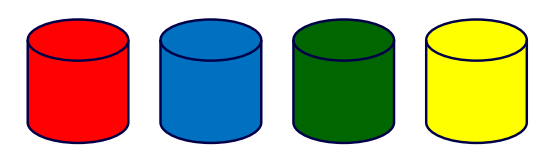
\includegraphics[width=\textwidth]{buildings.png}
\caption{Izgled zgradb}
\label{slika1}
\end{center}
\end{figure}


\pagebreak
\subsection{Zemljevid mesta}
\begin{figure}[!tbp]
  \centering
  \begin{minipage}[b]{0.2\textwidth}
	
\includegraphics[scale=0.6]{city.png}
	\caption{Skica mesta}
  \end{minipage}
  \hfill
  \begin{minipage}[b]{0.2\textwidth}
	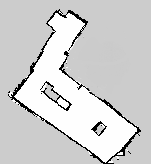
\includegraphics[scale=1]{robotMap.png}
	\caption{Mapa po kateri se je navigiral robot}
  \end{minipage}
\end{figure}



\section{\label{app-code}Programska koda}

TODO

\end{document}
